\chapter{Numerical Methods}

\section{Introduction}

In this section we want to introduce a part of the numerical methods, which were used in this thesis, for the performance of computations.
To solve the in chapter () introduced equations of motion it is necessary to use spatial and temporal discretization schemes, in order to
compute the time evolution of fluid system from the initial state.
Different approaches like finite element and volume methods exist, here we will introduce the use of finite difference stencils for the
spatial and a third order runge kutta method for the discretization in time.
The choice of these methods in combination with the use of cartesian grids is in particular time saving when performing computations on the gpu, as we
will see in chapter ().

\section{Finite Differencing Schemes}

We start with a brief introduction of finite difference methods,
the interested reader is referred to [], for a more general overview, on which this section is primarly based on.
Since the storage capacity and computation time of computers is limited it is necessary to approximate the contigious fluid domain  by a finite set of points,
such that the overall error maintains small.
To begin with we will fall back on the one dimensional case, where we want to discretize the operators

\begin{align}
    \pdn[]{x} \ , \ \pdn[^2]{x^2}
\end{align}

applied to the function $f:\mathbb{R}\rightarrow \mathbb{R} : x  \rightarrow f(x)$, on a domain $\Omega = \{x \in \mathbb{R} | 0 < x < L\}$.
For the discretization the simplest approach is to divide $\Omega$ into $N$ equidistant points $x_i= i\Delta x$ and $i=1..N$,
with the distance between two points given by $\Delta x = x_{i+1} - x_i = L/(N-1)$.
Local to a single point $x_i$, $f$ can be approximated with a taylor expansion.

\begin{align}
    f(x) = f(x_i) + \left(\pdn[f]{x} \right)_i (x - x_i) + \left(\pdn[^2f]{x^2}\right)_i \frac{(x-x_i)^2}{2!} + bla
\end{align}

Insert $x$ with $x_{i+1}$ or $x_{i-1}$ we obtain the forward and backward

 necgleting higher order terms, results in the following approximations for the first derivative.

\begin{align}
    \left(\pdn[f]{x}\right)_i &\approx \frac{f_{i+1} - f{i}}{\Delta x}\\
    \left(\pdn[f]{x}\right)_i &\approx \frac{f_{i} - f_{i-1}}{\Delta x}\\
    \left(\pdn[f]{x}\right)_i &\approx \frac{f_{i+1} - f_{i-1}}{2\Delta x}
\end{align}

\begin{figure}[!tpb]
  \centering
  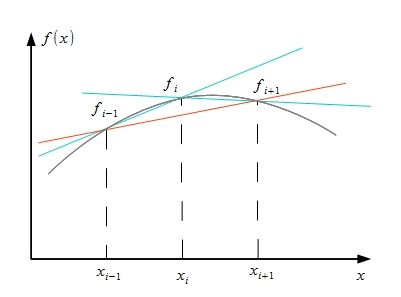
\includegraphics[width=0.6\textwidth]{gfx/numerik/fd_dummy.png}\label{fig:fd_schema}
  \caption{Approximation einer Funktion durch finite Differenznen}
\end{figure}

The first scheme is äquivalent to the definition of the first derivative, for $\Delta x \rightarrow 0$ and is also
denoted as forward difference, whereas the second scheme usually is referred to as backward difference.
The third approximation can be obtained by averaging over the first two approximations, and  is referred to as central difference.
The error resulting in the neglection of higher order terms in the taylor approximation, is denoted as the truncation error.
For the forward- and backward scheme this error is of first order, for the central scheme it is of second order.
All schemes are schematicaly shown in figure (), here the secord order central schemes results in the best approximationn.

\paragraph{Second Order}\mbox{}\\
\begin{align}
    \left(\pdn[f]{x}\right)_i &\approx \frac{f_{i+1} - f_{i-1}}{2\Delta x} \\
    \left(\pdn[^2f]{x^2}\right)_i &\approx \frac{f_{i+1} - 2 f_i +  f_{i-1}}{2\Delta x^2}
\end{align}
\paragraph{Fourth Order}\mbox{}\\
\begin{align}
    \left(\pdn[f]{x}\right)_i &\approx \frac{-f_{i+2} + 8f_{i+1} - 8f_{i-1} + f_{i-2}}{12\Delta x} \\
    \left(\pdn[^2f]{x^2}\right)_i &\approx \frac{-f_{i+2} + 16f_{i+1} -30f_i + 16f_{i-1} - f_{i-2}}{12\Delta x^2} \\
\end{align}

\newpage

\section{Runge Kutta Method}

For the temporal discretization the third-order low-storage Runge-Kutta scheme is used, first introduced by [Williamson].
Third order methods are often used for cfd-simulations, since they tend to stabilice numerical oscilltions in advection terms[].\\
We begin with considering the inital value problem.

\begin{align}
    \left(\pdn[f]{t}\right) = F(t, f(t)) ; f(t_0) = f_0
\end{align}

This differtial equation can be solved by integration, with the exact solution
\begin{align}
    f(t) = f(0) + \int_{t_n}^{t}F(t, f(t))dt
\end{align}
In the next step the integral is splitted into piecewiese integration, with time intervalls $[t^n, t^{n+1}]$.
\begin{align}
    f(t^{n+1}) = f(t) + \int_{t_n}^{t_{n+1}}F(t, f(t))dt
\end{align}

When using runge kutta methods, the function F(t, f(t)) is evaluated at $s$ different timesteps $\tau_i = t^n + \Delta t \alpha_i$,
furthermore for each $\tau$ a different weight parameter $b_i$ is used.V
The numerical computation of the integral is than given by [].

\begin{align}
    f(t^{n+1}) = f(t) + \Delta t \sum_{i=1}^s b_i k_i, k_i = F(t^n + \Delta t c_s, f^n + \Delta t \sum_{i=1}^{s-1}a_{si}k_i)
\end{align}

With the definition of $\sum c_i$, the runge kutta scheme of third order is festgelegt by the butcher tablau
By using taylor expansion and coefficient comparison, it can be shown that this  method converges at third order.


- In order to use as  so wenig speicher wie möglich williamson scheme
- 2 speicherstack für jede variable

\begin{align}
    S_1 = \delta t F(f^n ; f^(1) = f^n + \frac{S_1}{3}) \\
    S_1 = \delta t F(f^n ; f^(1) = f^n + \frac{S_1}{3}) \\
    S_1 = \delta t F(f^n ; f^(1) = f^n + \frac{S_1}{3}) \\
\end{align}


-stabilitätsregion

\section{Numerical Stability}\mbox{}\\

-beispiel erste abl dann zweit
-stabilität konstistenz - konvergenz etc
-verfahren höherer ordnung
-peclet zahl
-upwind schema



\newpage

\section{Artificial Kompressibility}
bewegungsgleichungen
druckterm diskussion
exkurs laplace gleichung
beispiel rayleigh benard diskretisierung

